% !TEX root = ../main.tex

\section{Introduction}
In this report, we attempt to validate the experimental results of ``BBR:
Congestion-based Congestion Control''~\cite{cardwell2016bbr}. We start
by looking at the goals, motivations and results from the BBR paper.

\para{Goals}
\emph{What was the original paper trying to solve?}

The original paper was trying to find a congestion control approach
that would stay as close as possible to optimal network operating point
in various network conditions. The network link is operating at the optimal
point when bandwidth utilization is maximized and latency and loss are
minimized, as shown by Leonard Kleinrock in 1979~\cite{kleinrock1979power}.
Furthermore, Jeffrey Jaffe proved that a distributed algorithm that converged
to this optimal point was an impossibility~\cite{jaffe1981flow}.

Loss-based congestion control operates by delivering full
bottleneck bandwidth at the cost of high delay and frequent packet loss.
Furthermore, Cardwell et. al. observed that because RTprop and BtlBw could
be inferred from traces, measurements over time could result in an
algorithm which converged with high probability to the optimal operating point.
BBR is an algorithm that seeks to converge to this optimal point.


\para{Motivation}
\emph{Why is the problem important/interesting?}

At a high level, the Internet could be moving data much more efficiently.
For example, cellular users can experience delays of seconds to minutes and
even multi-Gbps infrastructure may deliver data at a few Mbps when transmitting
over intercontinental distances. In addition, traditional congestion control
algorithms such as CUBIC have a tough time operating efficiently when there
is non-negligible packet loss in the network. This limitation comes from the
CUBIC's use of packet loss as a signal for congestion, which can unnecessarily
hinder throughput leading to poor performance.

Importantly, these limitations are not fundamental, but rather are a result
of particular implementation choices made in designing TCP congestion control.
In the original paper, the BBR authors seek to find an alternative to loss-based
congestion control, in an effort to mitigate many of these issues.

The problem is particularly interesting because, if successful, we will be able
to utilize the network infrastructure we have much more effectively, while
reducing latency experienced by users, without needing to upgrade or change
the network itself.

\para{Results}
\emph{What did the original authors find?}

The BBR paper describes a new form of congestion control that is based on actual
congestion in the network. The insight from the authors is that their
approach estimates bottleneck bandwidth and the minimum propagation delay
so as to be able to get as close as possible to the ideal operating point of
maximum bandwidth and minimal latency. We highlight several of the key
results below.

The first finding is that BBR can quickly adopt to changes in bottleneck link
bandwidth. During operation, BBR spends most of its time continuously probing
if more bandwidth has become available. Figure~\ref{fig:bbr3} shows BBR
reacting to a 2x increase and a 2x decrease to bottleneck bandwidth within
about 2 seconds.

\begin{figure}[h]
  \centering
  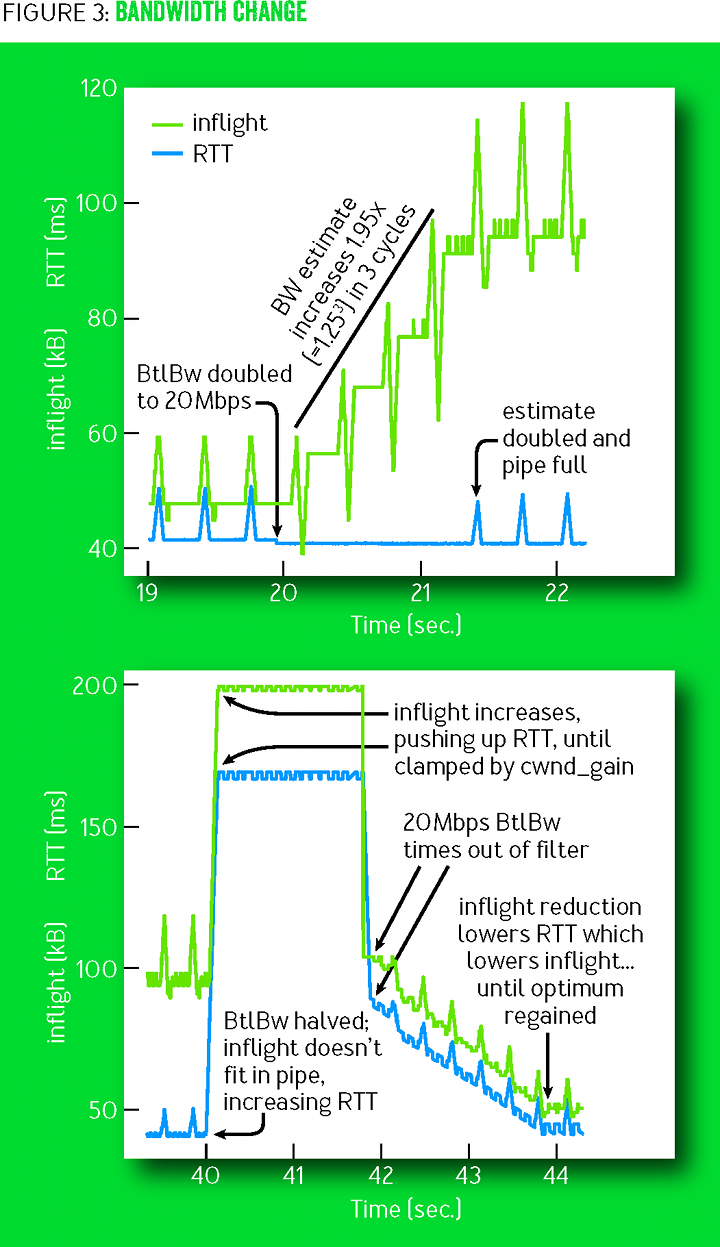
\includegraphics[height=9cm]{./img/bbr_fig3.png}
  \caption{BBR converges to new bottleneck bandwidth at exponential rate.
  This figure is from the original paper.}
  \label{fig:bbr3}
\end{figure}

The second finding is that BBR is able to avoid bloating router buffers
unnecessarily and thus is able to keep RTT at a minimum. This is in contrast to
CUBIC which continues to bloat a the bottleneck buffer until it observes a
packet loss event from overflowing the buffer. Figure~\ref{fig:bbr5} illustrates
hoe CUBIC and BBR behave in this regard.

\begin{figure}[h]
  \centering
  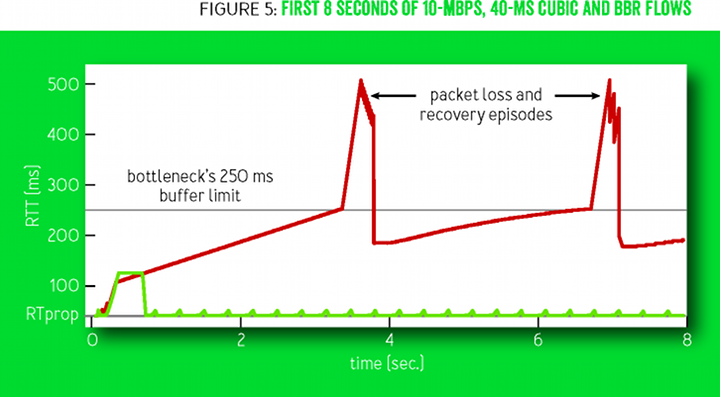
\includegraphics[width=1.0\columnwidth]{./img/bbr_fig5.png}
  \caption{BBR avoids bloating router buffer unlike CUBIC. Figure from original paper.}
  \label{fig:bbr5}
\end{figure}

Third, and one of the most interesting results, is that BBR outperforms
CUBIC for non-negligible loss rates. Figure~\ref{fig:bbr8} shows a graph
showing the performance comparison between BBR and CUBIC for varying loss rates.

\begin{figure}[h]
  \centering
  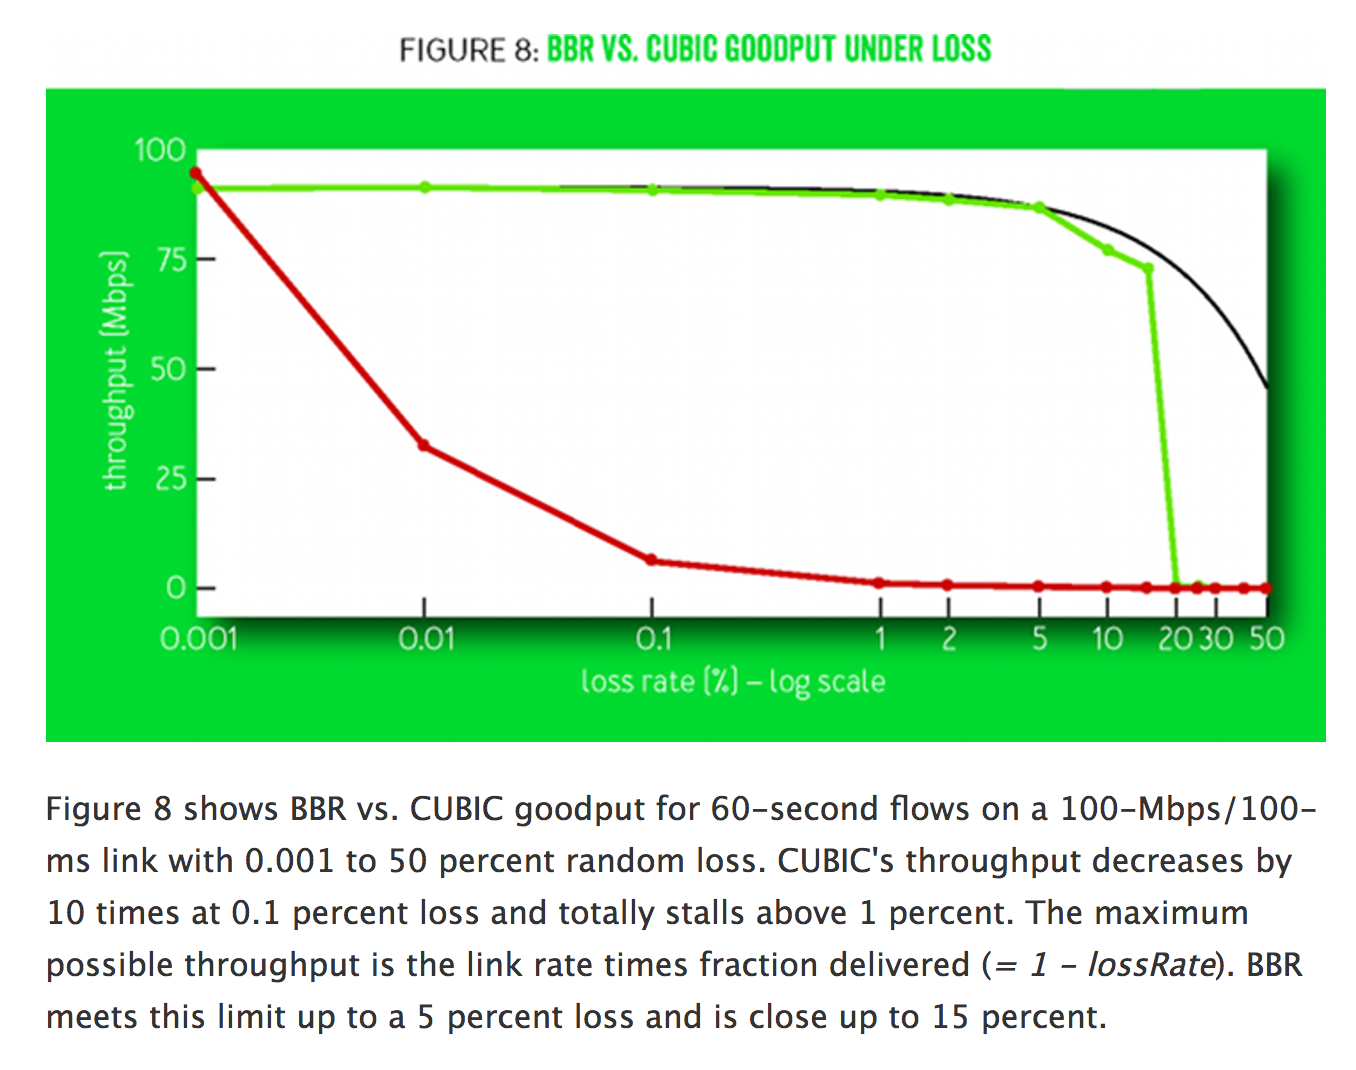
\includegraphics[width=1.0\columnwidth]{./img/bbr_fig8.png}
  \caption{Throughput vs loss rate comparing CUBIC vs BBR. Figure from original paper.}
  \label{fig:bbr8}
\end{figure}

The authors report that Google has had a very good experience deploying BBR
on B4---Google's data center to data center high-speed Wide Area Network built
primarily from commodity switches that have shallow/small memory buffers.
The limited amount of buffering means that there is the occasional packet
loss when there are bursts of incoming packets that arrive at the same time.
After switching to BBR from CUBIC, Google saw throughput improvements ranging
from $2\times$ to $25\times$.

Finally, the authors do acknowledge that there is still work to be done in terms
of how BBR interoperates with existing loss-based congestion controls algorithms
such as CUBIC. In cases where routers have large buffers, CUBIC senders can
drown out BBR. Gracefully mitigating this is an ongoing area of research.
